\documentclass[10pt,a4paper, margin=1in]{article}
\usepackage{fullpage}
\usepackage{amsfonts, amsmath, pifont}
\usepackage{amsthm}
\usepackage{graphicx}
\usepackage{float}

\usepackage{tkz-euclide}
\usepackage{tikz}
\usepackage{pgfplots}
\pgfplotsset{compat=1.13}

\usepackage{geometry}
 \geometry{
 a4paper,
 total={210mm,297mm},
 left=10mm,
 right=10mm,
 top=10mm,
 bottom=10mm,
 }
 % Write both of your names here. Fill exxxxxxx with your ceng mail address.
 \author{
  Aksoy, Aybüke\\
  \texttt{e2448090@ceng.metu.edu.tr}
  \and
  Varlı, Yiğit\\
  \texttt{e2381036@ceng.metu.edu.tr}
}

\title{CENG 384 - Signals and Systems for Computer Engineers \\
Spring 2022 \\
Homework 1}
\begin{document}
\maketitle



\noindent\rule{19cm}{1.2pt}

\begin{enumerate}

\item %write the solution of q1
    \begin{enumerate}
    % Write your solutions in the following items.
    \item We know that $\Bar{z} = x - jy$. We first need to find values of x and y by replacing the given equation with values of $z$ and $\Bar{z}$
    \[2(x + jy) - 9 = 4j - (x - jy)\]
    \[2x + 2jy - 9 = 4j - x + jy\]
    \[(3x-9) + j(y-4) = 0\]
    We find out that $x = 3$ and $y=4$. Thus $z = 3 + 4j$. \\\\
    i. $|z|$ means the length of complex vector. $|z| = \sqrt{a^2 + b^2}$ where $a=3$ and $b=4$. Thus $|z| = 5$ and $|z|^2 = 25$.\\
    ii. \begin{figure}[H]
     \centering
         \begin{tikzpicture}[scale=1.0]
           \begin{axis}[
           axis lines=middle,
           xlabel={$\hspace{10mm}Re\{z\}$},
           ylabel={$Im\{z\}$},%           xtick={-5, -3, -2, -1, ..., 1},
           ytick={-3, -2, -1, ..., 5},
           ymin=-1, ymax=5,
           xmin=-1, xmax=4,
         ]
           \addplot[thick, mark=] coordinates {(0,0) (3,4)};
           \filldraw [black] (3,4) circle (2pt);
           \end{axis}
         \end{tikzpicture}
         \caption{Plot of $z$}
         \label{fig:plotz}
     \end{figure}
     
    \item We know that $j^3 = -j$. Thus, we can change $-27j$ with $27j^3$. Our new equation will be $z^3 = 27j^3$. We can find out that:
    \[z = 3j\]
    Our complex number is in the form of $z = a + jb$, where $a = 0$ and $b = 3$. We know that $r = |z| = \sqrt{0^2 + 3^3} = 3$ and $\theta = arctan(b/a) = arctan(3/0) = \frac{\pi}{2}$. Thus, polar form of $z$ will be:
    \[z = 3e^{j\frac{\pi}{2}}\]
    \item To simplify, multiply $z$ with complex conjugate of $\sqrt{3} + j$.
    \[z = \frac{(1+j)(\sqrt{3}-j)^2}{(\sqrt{3}+j)(\sqrt{3}-j)} = \frac{(1+j)(2-2\sqrt{3}j)}{4}\]
    \[z = \frac{1+1\sqrt{3}}{2} +  j\frac{1-1\sqrt{3}}{2}\]
    We can calculate $|z| = \sqrt{a^2 + b^2}$ where $a = \frac{1 + 1\sqrt{3}}{2}$ and $b = \frac{1 - 1\sqrt{3}}{2}$. We can calculate the angle $\theta = arctan(b/a)$. From these equations:
    \begin{center}
        $|z| = \sqrt{2} = 1.4142$ and $\theta = -\frac{\pi}{12}$
    \end{center}\\
    \item Instead of $(1+j)^8$, we can write it as:
    \[((1+j)^2)^4 = (2j)^4 = 16\]
    Our new equation will be:
    \[z = -16e^{j\frac{\pi}{2}}\]
    In polar form, r cannot be negative. Thus, we need to handle minus sign with the angle. Instead of $\frac{\pi}{2}$, to get negative, we can use $-\frac{\pi}{2}$. Our z in polar form will be:
    \[z = 16e^{-j\frac{\pi}{2}}\]
    \end{enumerate}\vspace{5mm}
\item We know that the total energy and power of a continuous signal are as follows:
    \[E_x = \int_{-\infty}^{\infty} |x(t)|^2 dt \hspace{8mm} P_x = \lim_{T\to\infty} \frac{1}{2T} \int_{-T}^{T}|x(t)|^2 dt\]
    We know that the total energy and power of a discrete signal are as follows:
    \[E_x = \sum_{n=-\infty}^{\infty} |x[n]|^2 \hspace{8mm} P_x = \lim_{N\to\infty} \frac{1}{2N+1}\sum_{-N}^{N} |x[n]|^2\]
    \begin{enumerate}
    % Write your solutions in the following items.
    \item We can write $x[n] = nu[n]$ as follows:
    \[nu[n] =  \begin{cases} 
      n & n \geq 0 \\
      0 & n < 0 
   \end{cases}
    \]
    We can find the energy of this signal by using the formulas above. We can write signal as summation of two since it's piecewise. Thus, total energy becomes:
    \[E_x = \sum_{n=-\infty}^{-1} |0|^2 + \sum_{n=0}^{\infty} |n|^2 \to \infty\]
    Using the same approach, power of this signal becomes:
    \[P_X = \lim_{N\to\infty}\frac{1}{2N+1} (\sum_{-N}^{-1} |0|^2 + \sum_{0}^{N}|n|^2) =  \lim_{N\to\infty}\frac{1}{2N+1}\frac{N(N+1)(2N+1)}{6} \to \infty\]
    Since both of the calculations goes to $\infty$, this signal is neither a power signal nor an energy signal.\\
    \item We can write $x(t) = e^{-2t}u(t)$ as follows:
    \[e^{-2t}u(t) =  \begin{cases} 
      e^{-2t} & t \geq 0 \\
      0 & t < 0 
   \end{cases}
    \]
    We can find the energy of this signal using the same approach above but for continuous case:
    \[E_x = \int_{-\infty}^{0} |0|^2dt + \int_{0}^{\infty} |e^{-2t}|^2dt = 0 + (-\frac{1}{4}e^{-4t})\bigg|_0^\infty\]
    \[E_x = 0 + (-\frac{1}{4}e^{-\infty}) - (-\frac{1}{4}e^{0}) = 0.25\]
    By using the same approach, power of this signal becomes:
    \[P_x = \lim_{T\to\infty} \frac{1}{2T}(\int_{-T}^{0} |0|^2dt + \int_{0}^{T} |e^{-2t}|^2dt)\]
    We can just write power of signal as:
    \[P_x = \lim_{T\to\infty}\frac{E_x}{2T} = \lim_{T\to\infty}\frac{1/4}{2T} = 0\]
    Since $E_x < \infty$, this is an energy signal. However, due to $P_x = 0$, it is not a power signal.\\\\
    \end{enumerate}

\item %write the solution of q3 
  a) x(t+2) - Time Shifting:
  \begin{figure}[H]
     \centering
         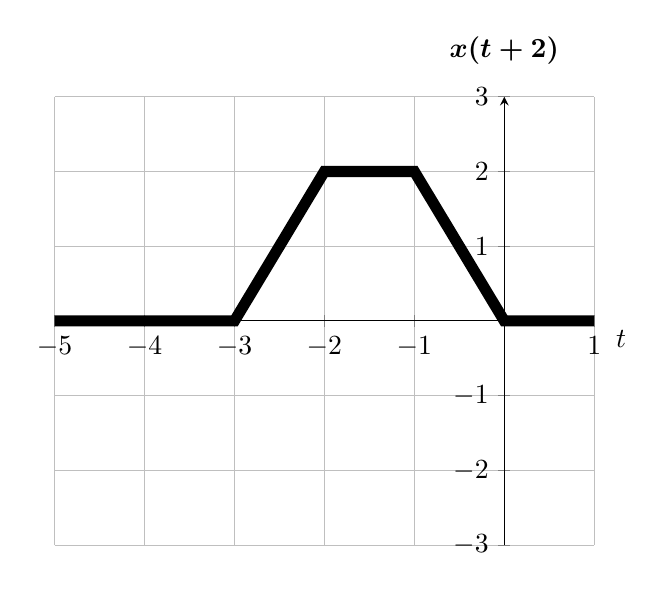
\begin{tikzpicture}[scale=1.0]
           \begin{axis}[
           axis lines=middle,
           xlabel={$t$},
           ylabel={$\boldsymbol{x(t+2)}$},%           xtick={-5, -3, -2, -1, ..., 1},
           ytick={-3, -2, -1, ..., 3},
           ymin=-3, ymax=3,
           xmin=-5, xmax=1,
           every axis x label/.style={at={(ticklabel* cs:1.05)}, anchor=north,},
           every axis y label/.style={at={(ticklabel* cs:1.05)}, anchor=south,},
           grid,
         ]
           \path[draw,line width=4pt] (-5,0) -- (-4,0) -- (-3,0) -- (-2,2) -- (-1,2) -- (0,0) -- (1,0);
           \end{axis}
         \end{tikzpicture}
         \caption{$t$ vs. $x(t+2)$.}
         \label{fig:fig6}
     \end{figure}
     
 \begin{filecontents}{fig6.dat}
  n   xn
 -5 0
 -4 0
 -3 0
 -2 2
 -1 2
 0 0
 1 0
 \end{filecontents}
 
   b) $x(-\frac{1}3 t+2)$ - Time Scaling:
  \begin{figure}[H]
     \centering
         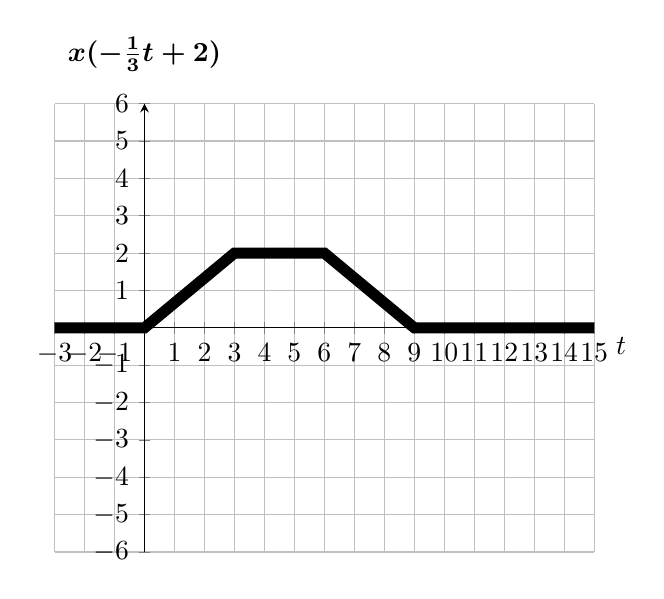
\begin{tikzpicture}[scale=1.0]
           \begin{axis}[
           axis lines=middle,
           xlabel={$t$},
           ylabel={$\boldsymbol{x(-\frac{1}3 t+2)}$},           
           xtick={-3, -2, -1,..., 15},
           ytick={-6,-5,-4,...,6},
           ymin=-6, ymax=6,
           xmin=-3, xmax=15,
           every axis x label/.style={at={(ticklabel* cs:1.05)}, anchor=north,},
           every axis y label/.style={at={(ticklabel* cs:1.05)}, anchor=south,},
           grid,
         ]
           \path[draw,line width=4pt] (-3,0) -- (0,0) -- (3,2) -- (6,2) -- (9,0) -- (12,0) -- (15,0);
           \end{axis}
         \end{tikzpicture}
         \caption{$t$ vs. $x(-\frac{1}3 t+2)$}
         \label{fig:fig7}
     \end{figure}
    
 \begin{filecontents}{fig7.dat}
  n   xn
 -5 0
 -4 0
 -3 0
 -2 2
 -1 2
 0 0
 1 0
 \end{filecontents}
    c) $\frac{1}2x(-\frac{1}3 t+2)$ - Amplitude Scaling:
  \begin{figure}[H]
     \centering
         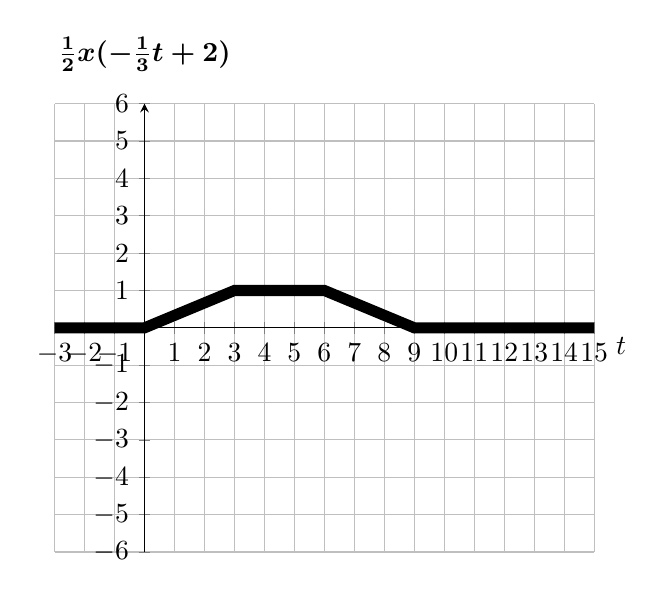
\begin{tikzpicture}[scale=1.0]
           \begin{axis}[
           axis lines=middle,
           xlabel={$t$},
           ylabel={$\boldsymbol{\frac{1}2x(-\frac{1}3 t+2)}$},           
           xtick={-3, -2, -1,..., 15},
           ytick={-6,-5,-4,...,6},
           ymin=-6, ymax=6,
           xmin=-3, xmax=15,
           every axis x label/.style={at={(ticklabel* cs:1.05)}, anchor=north,},
           every axis y label/.style={at={(ticklabel* cs:1.05)}, anchor=south,},
           grid,
         ]
           \path[draw,line width=4pt] (-3,0) -- (0,0) -- (3,1) -- (6,1) -- (9,0) -- (12,0) -- (15,0);
           \end{axis}
         \end{tikzpicture}
         \caption{$t$ vs. $\frac{1}2x(-\frac{1}3 t+2)$.}
         \label{fig:fig8}
     \end{figure}
    
 \begin{filecontents}{fig8.dat}
  n   xn
 -5 0
 -4 0
 -3 0
 -2 2
 -1 2
 0 0
 1 0
 \end{filecontents}
\item %write the solution of q4
    \begin{enumerate}
    % Write your solutions in the following items.
    \item %write the solution of q4a
    $x[-2n]:$
    \begin{filecontents}{fig1.dat}
    n   xn
    -1  1
    0 0
    1 -1
    2 0
    3 0
    \end{filecontents}

     \begin{figure}[H]
     \centering
     \begin{tikzpicture}[scale=1.0] 
       \begin{axis}[
           axis lines=middle,
           xlabel={$n$},
           ylabel={$x[-2n]$},
           xtick={ -2,-1, ...,4 },
           ytick={-2,-1, ..., 4},
           ymin=-2, ymax=4,
           xmin=-2, xmax=4,
           every axis x label/.style={at={(ticklabel* cs:1.05)}, anchor=west,},
           every axis y label/.style={at={(ticklabel* cs:1.05)}, anchor=south,},
           grid,
         ]
         \addplot [ycomb, black, thick, mark=*] table [x={n}, y={xn}] {fig1.dat};
       \end{axis}
     \end{tikzpicture}
     \caption{$n$ vs. $x[-2n]$.}
     \label{fig:fig1}
     \end{figure}
     
     $x[n-2]:$
        \begin{filecontents}{fig2.dat}
    n   xn
    -4 0
    -3 2
    -2 0
    -1 1
    0 -1
    1 -2
    2 0
    3 0
    4 1
    \end{filecontents}

     \begin{figure}[H]
     \centering
     \begin{tikzpicture}[scale=1.0] 
       \begin{axis}[
           axis lines=middle,
           xlabel={$n$},
           ylabel={$x[n-2]$},
           xtick={ -5, -4,  ..., 5},
           ytick={-4, -3, -2, -1, 0, 1, 2,3,4},
           ymin=-4, ymax=4,
           xmin=-5, xmax=5,
           every axis x label/.style={at={(ticklabel* cs:1.05)}, anchor=west,},
           every axis y label/.style={at={(ticklabel* cs:1.05)}, anchor=south,},
           grid,
         ]
         \addplot [ycomb, black, thick, mark=*] table [x={n}, y={xn}] {fig2.dat};
       \end{axis}
     \end{tikzpicture}
     \caption{$n$ vs. $x[n-2]$.}
     \label{fig:fig2}
     \end{figure}
    $x[-2n]+x[n-2]:$
     \begin{filecontents}{fig3.dat}
    n   xn
    -4 0
    -3 2 
    -2 0
    -1 2
    0 -1
    1 -3
    2 0
    3 0
    4 1
    \end{filecontents}

     \begin{figure}[H]
     \centering
     \begin{tikzpicture}[scale=1.0] 
       \begin{axis}[
           axis lines=middle,
           xlabel={$n$},
           ylabel={$x[-2n]+x[n-2]$},
           xtick={-4,-3, ...,4},
           ytick={-3,-2, ...,3},
           ymin=-3, ymax=3,
           xmin=-4, xmax=4,
           every axis x label/.style={at={(ticklabel* cs:1.05)}, anchor=west,},
           every axis y label/.style={at={(ticklabel* cs:1.05)}, anchor=south,},
           grid,
         ]
         \addplot [ycomb, black, thick, mark=*] table [x={n}, y={xn}] {fig3.dat};
       \end{axis}
     \end{tikzpicture}
     \caption{$n$ vs. $x[-2n]+x[n-2]$.}
     \label{fig:fig3}
     \end{figure}
     

    \item %write the solution of q4b
    $x[-2n]+x[n-2] = 2\delta[n+3]+2\delta[n+1]-\delta[n]-3\delta[n-1]+\delta[n-4]$
    \end{enumerate}

\item %write the solution of q5
    \begin{enumerate}   
    % Write your solutions in the following items.
    \item If the signal is periodic, we have a fundamental period $T_0$ such that $x(t) = x(t + T_0)$. Using this information, we can write the equation below:
    \[\frac{e^{j3t}}{-j} = \frac{e^{j3t}e^{j3T_0}}{-j}\]
    To maintain equality, we need to have $e^{j3T_0} = 1$. We can express it with Euler's formula:
    \[e^{j3T_0} = cos(3T_0) + jsin(3T_0) =  1\]
    We do not have any imaginary part, so $sin(3T_0) = 0$ and  $cos(3T_0) = 1$. 
    \[3T_0 = 2\pi k\]
    \[T_0 = 2\pi /3\]
    \item If the signal is periodic, we have a fundamental period $N_0$ such that $x[n] = x[n + N_0]$. Using this information, we can write the equation below:
    \begin{center}
        \begin{math}
            \frac{1}{2}sin[\frac{7\pi}{8}n] + 4cos[\frac{3\pi}{4}n - \frac{\pi}{2}] = \frac{1}{2}sin[\frac{7\pi}{8}n + \frac{7\pi}{8}N_0] + 4cos[\frac{3\pi}{4}n + \frac{3\pi}{4}N_0 - \frac{\pi}{2}]
        \end{math}
    \end{center}
    To satisfy normal period of sin and cos, we need to have:
    \[\frac{7\pi}{8}N_0 = 2\pi k_1 \hspace{8mm} \frac{3\pi}{4}N_0 = 2\pi k_2\]
    \[N_0 = \frac{16k_1}{7} \hspace{8mm} N_0 = \frac{8k_2}{3}\]
    We can find smallest common integer value of $N_0 = 16$.
    \end{enumerate}

\item %write the solution of q6
    \begin{enumerate}
    % Write your solutions in the following items.
    \item %write the solution of q6a
    A continuous time signal x(t) is considered an even signal if it satisfies the condition:
    \[x(t)=x(-t)\]
    We need to find x(-t) by applying time scaling on x(t) with -1.
    \begin{figure}[H]
     \centering
         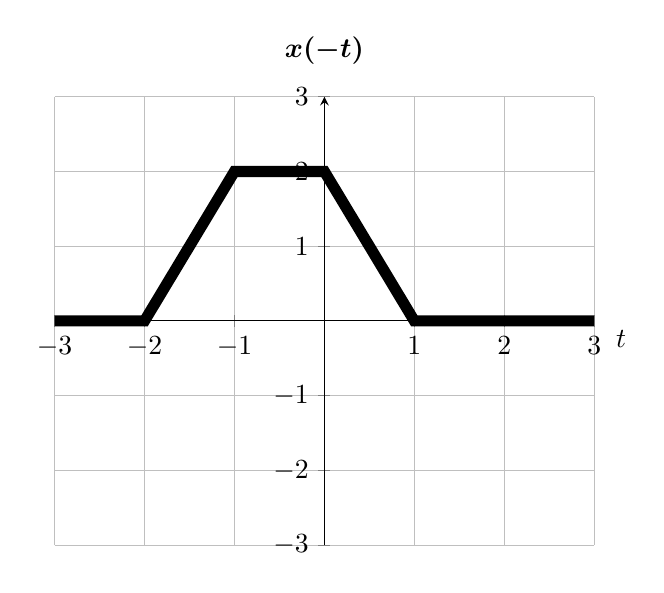
\begin{tikzpicture}[scale=1.0]
           \begin{axis}[
           axis lines=middle,
           xlabel={$t$},
           ylabel={$\boldsymbol{x(-t)}$},%           
           xtick={-3, -2, -1, ..., 1,2,3},
           ytick={-3, -2, -1, ..., 3},
           ymin=-3, ymax=3,
           xmin=-3, xmax=3,
           every axis x label/.style={at={(ticklabel* cs:1.05)}, anchor=north,},
           every axis y label/.style={at={(ticklabel* cs:1.05)}, anchor=south,},
           grid,
         ]
           \path[draw,line width=4pt] (-3,0) -- (-2,0) -- (-1,2) -- (0,2) -- (1,0) -- (2,0) -- (3,0);
           \end{axis}
         \end{tikzpicture}
         \caption{$t$ vs. $x(-t)$.}
         \label{fig:fig8}
     \end{figure}
     
 \begin{filecontents}{fig8.dat}
  n   xn
 -5 0
 -4 0
 -3 0
 -2 2
 -1 2
 0 0
 1 0
 \end{filecontents}
     
    Since the graphs of x(t) and x(-t) are different, we can directly say that x(t) is not equal to x(-t). Hence, x(t) is not even as it does not satisfy the condition. \\
    
    A continuous time signal x(t) is called an odd signal if it satisfies the condition:
     \[x(-t)=-x(t)\]
     \[x(t)=-x(-t)\]
    We need to find -x(-t) by applying time scaling on x(t) with -1 and by applying amplitude scaling with -1. 
    .  \begin{figure}[H]
     \centering
         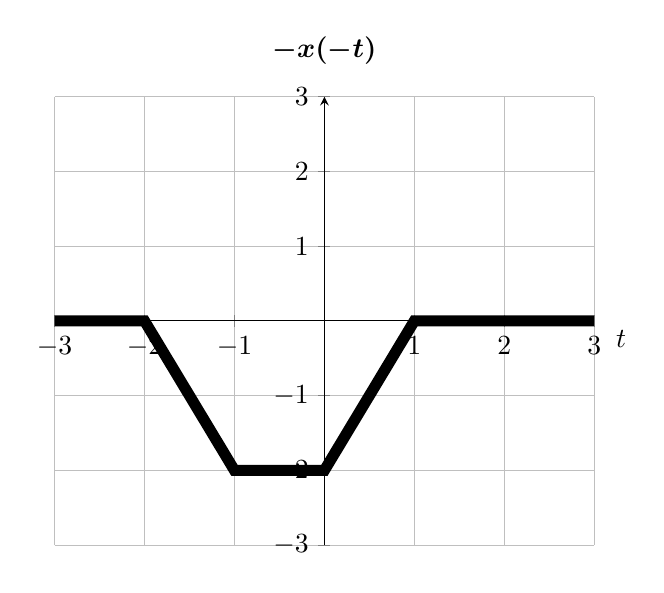
\begin{tikzpicture}[scale=1.0]
           \begin{axis}[
           axis lines=middle,
           xlabel={$t$},
           ylabel={$\boldsymbol{-x(-t)}$},%           
           xtick={-3, -2, -1, ..., 1,2,3},
           ytick={-3, -2, -1, ..., 3},
           ymin=-3, ymax=3,
           xmin=-3, xmax=3,
           every axis x label/.style={at={(ticklabel* cs:1.05)}, anchor=north,},
           every axis y label/.style={at={(ticklabel* cs:1.05)}, anchor=south,},
           grid,
         ]
           \path[draw,line width=4pt] (-3,0) -- (-2,0) -- (-1,-2) -- (0,-2) -- (1,0) -- (2,0) -- (3,0);
           \end{axis}
         \end{tikzpicture}
         \caption{$t$ vs. $-x(-t)$.}
         \label{fig:fig9}
     \end{figure}
     
 \begin{filecontents}{fig9.dat}
  n   xn
 -5 0
 -4 0
 -3 0
 -2 2
 -1 2
 0 0
 1 0
 \end{filecontents}
    Since the graphs of x(t) and -x(-t) are different, we can directly say that x(t) is not equal to -x(-t). Hence, x(t) is not odd as it does not satisfy the condition. \\
    
    Therefore, we can say that x(t) is neither even nor odd. \\
    
    
    \item %write the solution of q6b
    Any signal can be written as the sum of an even signal and odd signal where $x_e(t)$ is the even part and $x_o(t)$ is the odd part. 
    \[x(t)=x_e(t)+x_o(t)\]
    To find these even and odd parts of the signal:
     \[x(t)+x(-t)=x_e(t)+x_o(t)+x_e(t)-x_o(t)\]  by the definition of even and odd signals.
      \[x_e(t)=\frac{1}2(x(t)+x(-t))\]
    \[x(t)-x(-t)=(x_e(t)+x_o(t))-(x_e(t)-x_o(t))\]  by the definition of even and odd signals.
    \[x_0(t)=\frac{1}2(x(t)-x(-t))\]\\
    We have already found x(-t) and -x(-t) in part a. Therefore, we can use those graphs to draw the even and odd parts of x(t).\\
    
    $x_e(t)=\frac{1}2(x(t)+x(-t))$:
    \begin{figure}[H]
     \centering
         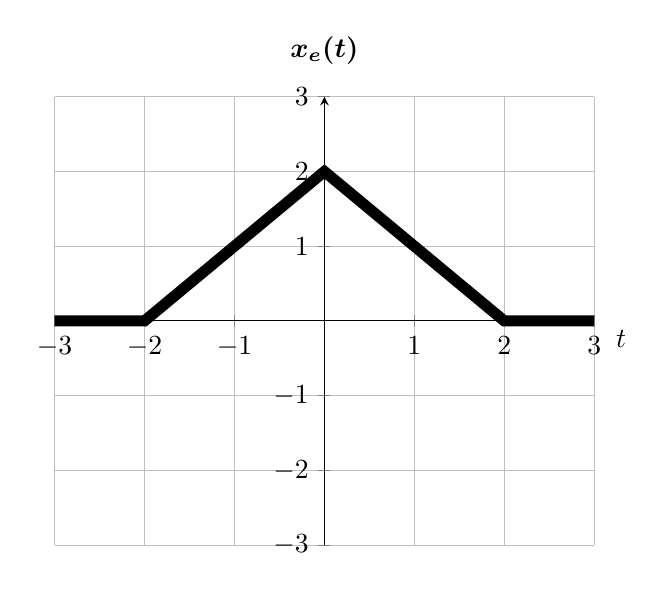
\begin{tikzpicture}[scale=1.0]
           \begin{axis}[
           axis lines=middle,
           xlabel={$t$},
           ylabel={$\boldsymbol{x_e(t)}$},%           
           xtick={-3, -2, -1, ..., 1,2,3},
           ytick={-3, -2, -1, ..., 3},
           ymin=-3, ymax=3,
           xmin=-3, xmax=3,
           every axis x label/.style={at={(ticklabel* cs:1.05)}, anchor=north,},
           every axis y label/.style={at={(ticklabel* cs:1.05)}, anchor=south,},
           grid,
         ]
           \path[draw,line width=4pt] (-3,0) -- (-2,0) -- (-1,1) -- (0,2) -- (1,1) -- (2,0) -- (3,0);
           \end{axis}
         \end{tikzpicture}
         \caption{$t$ vs. $x_e(t)$.}
         \label{fig:fig10}
     \end{figure}
     
 \begin{filecontents}{fig10.dat}
  n   xn
 -5 0
 -4 0
 -3 0
 -2 2
 -1 2
 0 0
 1 0
 \end{filecontents}
 $x_o(t)=\frac{1}2(x(t)+(-x(-t)))$:
    \begin{figure}[H]
     \centering
         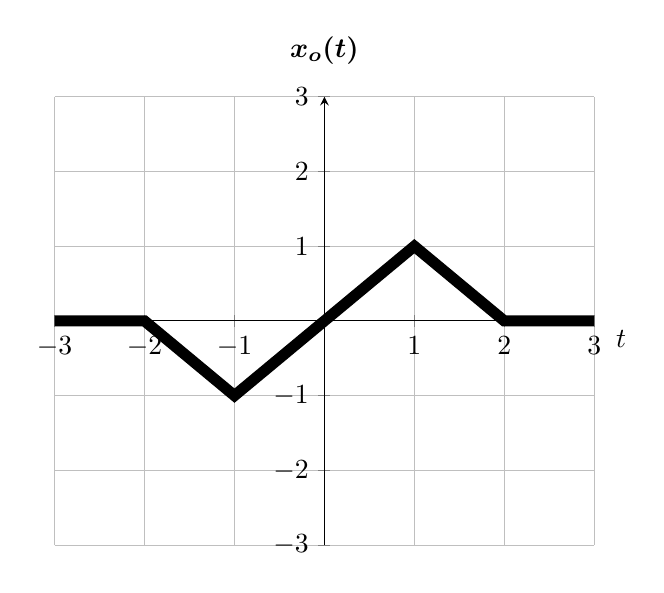
\begin{tikzpicture}[scale=1.0]
           \begin{axis}[
           axis lines=middle,
           xlabel={$t$},
           ylabel={$\boldsymbol{x_o(t)}$},%           
           xtick={-3, -2, -1, ..., 1,2,3},
           ytick={-3, -2, -1, ..., 3},
           ymin=-3, ymax=3,
           xmin=-3, xmax=3,
           every axis x label/.style={at={(ticklabel* cs:1.05)}, anchor=north,},
           every axis y label/.style={at={(ticklabel* cs:1.05)}, anchor=south,},
           grid,
         ]
           \path[draw,line width=4pt] (-3,0) -- (-2,0) -- (-1,-1) -- (0,0) -- (1,1) -- (2,0) -- (3,0);
           \end{axis}
         \end{tikzpicture}
         \caption{$t$ vs. $x_o(t)$.}
         \label{fig:fig10}
     \end{figure}
     
 \begin{filecontents}{fig10.dat}
  n   xn
 -5 0
 -4 0
 -3 0
 -2 2
 -1 2
 0 0
 1 0
 \end{filecontents}
    
    
    \end{enumerate}    
    
\item %write the solution of q7
    \begin{enumerate}
    % Write your solutions in the following items.
    \item We can write x(t) as:
    \[x(t) = 3u(t+3) - 3u(t+1) + 2u(t-2) - 4u(t-4) + 3u(t-6)\]
    \item We know that:
    \[\frac{du(t)}{dt} = \delta(t)\]
    Thus, we can write $\frac{dx(t)}{dt}$ as:
    \[\frac{dx(t)}{dt} = 3\delta(t+3) - 3\delta(t+1) + 2\delta(t-2) - 4\delta(t-4) + 3\delta(t-6)\]
    
    \begin{filecontents}{fig4.dat}
    n   xn
    -3  3
    2   2
    6   3
    \end{filecontents}
    
    \begin{filecontents}{fig42.dat}
     n  xn
     -1 -3
     4 -4
    \end{filecontents}

     \begin{figure}[h!]
     \centering
     \begin{tikzpicture}[scale=1.0] 
       \begin{axis}[
           axis lines=middle,
           xlabel={$t$},
           ylabel={$\frac{dx(t)}{dt}$},
           xtick={ -5, -4,  ..., 7},
           ytick={-4, -3, -2, -1, ..., 4},
           ymin=-4, ymax=4,
           xmin=-5, xmax=7,
           every axis x label/.style={at={(ticklabel* cs:1.05)}, anchor=west,},
           every axis y label/.style={at={(ticklabel* cs:1.05)}, anchor=south,},
           grid,
         ]
         \addplot [ycomb, black, thick, mark=triangle] table [x={n}, y={xn}] {fig4.dat};
         \addplot [ycomb, black, thick, mark=triangle, mark options={rotate=180}] table [x={n}, y={xn}] {fig42.dat};
       \end{axis}
     \end{tikzpicture}
     \caption{$t$ vs. $\frac{dx(t)}{dt}$}
     \label{fig:fig4}
     \end{figure}
    \end{enumerate}
    
\item %write the solution of q8
    \begin{enumerate}
    % Write your solutions in the following items.
    \item 
    \begin{itemize}
        \item The system has memory since it depends on past or future values of input. (e.g. $y[1] = x[0]$)
        \item The system is stable because our output signal depends only on the input signal. If we assume $x[2n-2] < A$, where A is finite number, output signal is also bounded.
        \item The system is not casual since it depends on future values of input for $n>2$. (e.g. $y[3] = x[4]$)
        \item The system is linear since it satisfies the superposition rule. Assume the followings:
        \[y_1[n] = x_1[2n-2]\]
        \[y_2[n] = x_2[2n-2]\]
        Then, we can see that the superposition holds:
        \[x_3[2n-2] = ax_1[2n-2] + bx_2[2n-2]\]
        \[y_3[n] = x_3[2n-2]\]
        \[y_3[n] = ax_1[2n-2] + bx_2[2n-2]\]
        \[y_3[n] = ay_1[n] + by_2[n]\]
        \item We know that a system is invertible if different inputs give different outputs. Since the output of the system depends only on the input, it is clear that different inputs will lead to different outputs. We can write $h^{-1}$ as:
        \[h^{-1} = y[\frac{n}{2} + 1] = x[n]\]
        \item The system is not time-invariant since delay of $N$ in the system:
        \[y[n + N] = x[2(n +N) -2]\]
        \[x[2n -2 + 2N] \neq x[2n-2 + N]\]
    \end{itemize}
    \item 
    \begin{itemize}
        \item The system has memory since it depends on past or future values of input (e.g. y(2) = 2x(0))
        \item The system is not stable. Assume that $x(\frac{t}{2} -1) < A$, where $A$ is finite constant. Our system will be $y(t) = tA$, and as time goes to infinity, output signal will approach to infinity.
        \item The system is not causal since output signal depends on the future values of input signal for $t < -2$. (e.g. y(-4) = -4x(-3))
        \item The system is linear since superposition holds:
        \[y(t) = h\{x(\frac{t}{2} -1)\}\]
        \[y_1(t) = tx_1(\frac{t}{2} -1) \hspace{8mm} y_2(t) = tx_2(\frac{t}{2} -1)\]
        \[t(ax_1(\frac{t}{2} -1)) + t(bx_2(\frac{t}{2} -1)) = ay_1(t) + by_2(t)\]
        \[t(ax_1(\frac{t}{2} -1) + bx_2(\frac{t}{2} -1)) = h\{ax_1(\frac{t}{2} -1) + bx_2(\frac{t}{2} -1)\}\]
        \[h\{ax_1(\frac{t}{2} -1) + bx_2(\frac{t}{2} -1)\} = h\{ax_1(\frac{t}{2} -1)\} + h\{bx_2(\frac{t}{2} -1)\}\]
        \[h\{ax_1(\frac{t}{2} -1)\} + h\{bx_2(\frac{t}{2} -1)\} = ah\{x_1(\frac{t}{2} -1)\} + bh\{x_2(\frac{t}{2} -1\}\]
        \item The system is not invertible since for $t=0$ any input signal leads to 0 which means it is not 1-1.
        \item The system is not time-invariant since delay of $T$ in the system:
        \[y(t+T) = (t+T)x(\frac{t+T}{2} - 1) \neq tx(\frac{t}{2} -1 + T)\]
    \end{itemize}
    \end{enumerate}  

\end{enumerate}

%\begin{figure}[h!]
%     \centering
%         \begin{tikzpicture}[scale=1.0]
%           \begin{axis}[
%           axis lines=middle,
%           xlabel={$t$},
%           ylabel={$\boldsymbol{x(t)}$},%           xtick={-4, -3, -2, -1, ..., 4},
%           ytick={-3, -2, -1, ..., 3},
%           ymin=-3, ymax=3,
%           xmin=-4, xmax=4,
%           every axis x label/.style={at={(ticklabel* cs:1.05)}, anchor=north,},
%           every axis y label/.style={at={(ticklabel* cs:1.05)}, anchor=south,},
%           grid,
%         ]
%           \path[draw,line width=4pt] (-4,0) -- (-3,0) -- (-2,0) -- (-1,1) -- (1,1) -- (1,0) -- (3,0) -- (4,0);
%           \end{axis}
%         \end{tikzpicture}
%         \caption{$t$ vs. $x(t)$.}
%         \label{fig:fig5}
%     \end{figure}
    
 \begin{filecontents}{fig5.dat}
  n   xn
  -1  1
  0   0
  1   0  
  2   -2
  3   0
  4   3 
  5   0
  6   0
  7   -4
 \end{filecontents}

% \begin{figure}[h!]
%     \centering
%     \begin{tikzpicture}[scale=1.0] 
%       \begin{axis}[
%           axis lines=middle,
%           xlabel={$n$},
%           ylabel={$\boldsymbol{x[n]}$},
%           xtick={ -1, 0,  ..., 7},
%           ytick={-4, -3, -2, -1, ..., 4},
%           ymin=-4, ymax=4,
%           xmin=-1, xmax=7,
%           every axis x label/.style={at={(ticklabel* cs:1.05)}, anchor=west,},
%           every axis y label/.style={at={(ticklabel* cs:1.05)}, anchor=south,},
%           grid,
%         ]
%         \addplot [ycomb, black, thick, mark=*] table [x={n}, y={xn}] {fig2.dat};
%       \end{axis}
%     \end{tikzpicture}
%     \caption{$n$ vs. $x[n]$.}
%     \label{fig:fig2}
% \end{figure}

\end{document}

